\documentclass[11pt]{article}
\usepackage[utf8]{inputenc}
\usepackage[french]{babel}
\usepackage{amsmath, amssymb, amsfonts}
\usepackage{graphicx}
\usepackage{hyperref}
\usepackage{cite}
\usepackage{geometry}
\geometry{a4paper, margin=1in}
\usepackage{parskip}

%\setlength{\parindent}{0pt}

\title{Apprentissage Continu des Dynamiques d'un Double Pendule par World Model Hamiltonien Constraint}
\author{Axel Bröns}
\date{\today}

\begin{document}

\maketitle
%
% \begin{abstract}
% Ce papier présente une approche de World Model continu pour la prédiction de l'état d'un double pendule (système chaotique type \texttt{Acrobot-v1}) directement à partir de pixels. Le modèle combine un auto-encodeur convolutif pour la perception visuelle, un réseau de neurones hamiltonien (HNN) pour capturer les lois de conservation d'énergie physique, et un intégrateur d'équations différentielles ordinaires (Neural ODE) pour la modélisation en temps continu. Pour forcer l'apprentissage de variables latentes physiquement interprétables (positions et moments canoniques), j'introduis des fonctions de coût de cohérence des coordonnées et de conservation d'énergie. Les résultats montrent que cette approche conserve mieux l'énergie à long terme et apprend un espace de phase structuré cohérent avec la mécanique classique.
% \end{abstract}

\section{Introduction}
\label{sec:intro}
On aperçoit le succès des World Models à travers de plusieurs papiers remarquables comme par exemple la famille des JEPA et LeWorldModel de Yann Le Cun. Le problème notable de ces modèles est l'apprentissage des dynamiques de transitions en temps discret sans contraintes physiques (qui est très important en robotique de précisions ou prévisions précises). Les trajectoires peuvent alors devenir irréalistes sur des systèmes physiques rigides. Ainsi mon approche vise à implémenter les principes fondamentaux de physique (mécanique hamiltonienne) avec la perception visuelle d'un World Model tout en modélisant de manière continu à l'aide des Neural ODEs. Dans cette étude, on va principalement se concentrer sur le double pendule (Acrobot-v1 de Gymnasium) qui est un système totalement chaotiques et non-linéaire qui est un réel challenge et cool à prédire ! Le système peut très bien changer, et libre à vous de choisir votre meilleur environnement. Le but de ce papier est d'expliquer de manière claire l'intuition derrière cette approche et comprendre comment le modèle peut apprendre la physique qui nous entoure !

% \begin{itemize}
%     \item \textbf{Contexte :} Succès des modèles de monde (\textit{World Models}) \cite{ha2018worldmodels} dans l'apprentissage par renforcement visuel et la planification de trajectoires.
%     \item \textbf{Problématique :} Les modèles de monde standards apprennent souvent des dynamiques de transition en temps discret sans contrainte physique. Cela peut mener à des dérives énergétiques ou des trajectoires irréalistes sur des systèmes physiques rigides.
%     \item \textbf{Objectif de l'approche :} Combiner la perception visuelle à base de pixels avec des principes physiques fondamentaux (mécanique hamiltonienne) modélisés en temps continu à l'aide des Neural ODEs \cite{chen2018neural}.
%     \item \textbf{Cas d'étude :} Le double pendule (Acrobot-v1 de Gymnasium \cite{gymnasium_2025}), un système non-linéaire et chaotique.
% \end{itemize}

\section{Mécanique Hamiltonienne}\label{sec:hamilton}
La première partie est là pour expliquer d'abord comment fonctionne la mécanique hamiltonienne et comment elle est intégrée dans un réseau de neurones. 

\subsection{Théorie}
La mécanique hamiltonienne, inventée par Hamilton en 1833, est une reformulation de la mécanique classique. Elle a différent domaine d'application et a notamment permis à l'élaboration théorique de la mécanique quantique. 

\paragraph{Mécanique Lagrangienne}
La mécanique hamiltonienne vient de la mécanique Lagrangienne. Concrètement les équations de mouvements d'un système à $N$ degrés de liberté dépendent des coordonnées généralisées $\{q_i\}_{i=1,...,N}$ et des vitesses correspondantes, $\{\dot q_i\}_{i=1,...,N}$ où $\dot q_i = \frac{dq_i}{dt}$. 

Le lagrangien peut donc s'écrire formellement comme une fonction : $\mathcal{L}(q_i, \dot q_i, t)$. les variables indexées représentant les $N$ variables de ce type.

En mécanique hamiltonienne, le moment conjugués $p_i$ est relié à la coordonnée généralisées $q_i$ (en gros la position si on veut rester simple) par : 
\begin{equation}\label{eq:position}
    p_i = \frac{\partial \mathcal{L}}{\partial \dot q_i}
\end{equation}
où $\mathcal {L}$ est le lagrangien et $\dot {q}_{i}$ est une vitesse généralisée définie comme la dérivée par rapport au temps de $q_{i}$
En coordonnées cartésiennes, les moments conjugués sont équivalents aux quantités de mouvement, alors qu'en coordonnées polaires ils correspondent aux moments angulaires.

\textit{Exemple :} Le moment conjugué d'un pendule simple est : 
\[
p_{\theta} = ml^2 \dot{\theta}
\]
avec $m$ la masse du pendule, $l$ sa longueur, $\dot \theta$ la vitesse angulaire, $\dot \theta = \frac{d \theta}{dt}$, avec $\theta$ l'angle que fait le pendule avec la verticale descendante.

\paragraph{Mécanique Hamiltonienne} 
Par définition, on a le hamiltonien $\mathcal{H}$ la transformée de Legendre du lagrangien :
\begin{equation}\label{eq:hamiltonien}
    \mathcal{H}(q_i, p_i, t) = \sum_{k}^{N} \dot q_k p_k - \mathcal{L}(q_i, \dot q_i, t)
\end{equation}

Si les équations qui définissent les coordonnées généralisées sont indépendantes du temps $t$, on peut montrer que $\mathcal {H}$ est égal à l'énergie totale $E$, elle-même étant égale à la somme de l'énergie cinétique T et de l'énergie potentielle $V$. Alors on aura : $\mathcal{H} = E = T + V$. 

Les parties qui vont nous être utile pour notre réseau de neurones sont les équations canoniques d'Hamilton.  

Sous forme differentielle $d\mathcal{H}$ et en utilisant la définition des moments conjugués donnée précédemment et les équations d'Euler Lagrange traduisant le principe de l'action minimale du lagrangien, on obtient les équations du mouvement de Hamilton, dites équations canoniques de Hamilton on retombe : 

\begin{equation}\label{eq:diff}
    \frac{dq_i}{dt} = \frac{\partial \mathcal{H}}{\partial p_i} \quad \text{et} \quad \frac{dp_i}{dt} = - \frac{\partial \mathcal{H}}{\partial q_i}
\end{equation}

On peut noter maintenant $\mathcal{S}_{\mathcal{H}} = \{\frac{\partial \mathcal{H}}{\partial p_i} , - \frac{\partial \mathcal{H}}{\partial q_i} \}$ l'évolution du temps du système. Il faut voir $\mathcal{S}_{\mathcal{H}}$ comme un champs de vecteur sur les entrées $\mathcal{H}$. On appelle ce genre de champs de vecteur les "symplectic gradient". Concrètement, ce type de champs est super important car il permet au gradient de garder un output totalement constant (et ainsi garder l'energe total du système constant). On peut noter aussi que les équations d'Hamilton sont des équations différentielles du premier ordre (à l'inverse des équations différentielles de Lagrange qui sont elles, d'ordre 2).

Les équations de Newton permettent également la prédiction le mouvement d'un pendule mais l'avantage d'utiliser les équations Hamiltonienne concerne le degré de liberté qui peut être généralisé à $N$ degrés de liberté (par exemple, le corps humain possède + de 200 degrés de liberté). 

Le gros avantage de travailler avec des équations différentielles est la continuité de la prédiction.

\section{World Model avec HNN et Neural ODE}
Concernant l'architecture d'un World Model, il se divise généralement en trois composants principaux : la vision, la mémoire, et le contrôleur \cite{ha2018worldmodels}. Toutes les planifications et les prédictions se font dans l'espace latent.

\begin{figure}\label{fig:architecture}
 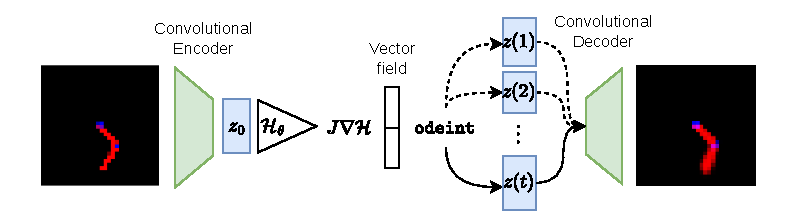
\includegraphics[width=\linewidth]{images/pipeline-wm2.pdf}
 \caption{Architecture général du modèle}
\end{figure}

Pour comprendre l'architecture du modèle, il faut essayer de comprendre les différentes étapes clés du modèle qui vont naturellement faire sens si vous avez compris la partie~\ref{sec:hamilton}. On peut voir les étapes séquentiellement dans la figure~\ref{fig:architecture}.

\paragraph{1ère étape (obtention de $z_0$):}
La première étape consiste à encoder l'information à l'aide d'un simple encodeur convolutionel. Pour ça, on prend 3 images successives et on les passe directement dans l'encodeur. Les images arrivent en $32 \times 32$ et possèdent 9 canaux (3 images avec chaque pixels en RGB donc $3 \times 3$) et le but est de les flatten en un vecteur de dimension $d' = 1024$. (précisément on a : $(32 \times 32 \times 9) \rightarrow (16 \times 16 \times 32) \rightarrow (8 \times 8 \times 64) \rightarrow (4 \times 4 \times 128) \rightarrow (2 \times 2 \times 256) = 1024$). Maintenant on passe une simple couche linéaire pour avoir de l'espace latent $z_0 \in \mathbb{R}^{2d}$ avec $2d = 16$. Pourquoi 16 ? Parce qu'on découpe l'espace latent en deux. D'une part le vecteur position $\mathbf{q}_0$ et l'autre part, le vecteur momentum $\mathbf{p}_0$, tous les deux de dimension $\mathbb{R}^8$. On a alors juste à les concaténer pour avoir notre espace latent $z_0 = [\mathbf{q}_0,\mathbf{p}_0]^{\top}$.

\paragraph{2ème étape (obtention de $\mathcal{H}_{\theta}$):}
Maintenant le but de cette étape est de récupérer l'energie totale du système. Vu qu'on sait que l'energie totale est ni plus ni moins que l'hamiltonien $\mathcal{H}$ (représente un scalaire dans l'équation~\ref{eq:hamiltonien}). L'intuition sera de prendre ce scalaire pour avoir ensuite la gamme des dérivées partielles~\ref{eq:diff}, permettant de faire apparaître le $dt$ pour ensuite faire une équa diff. Pour obtenir $\mathcal{H}_{\theta}$ on a juste à entraîner un MLP qui prend en input  $z_0 \in \mathbb{R}^{2d}$, ensuite de passer dans 2 hidden layers de dimension 200 pour ensuite finir en output de 1 (scalaire à la fin). Le tout séparé par une fonction d'activation \texttt{Tanh} pour garder au maximum la continuité (fonction de classe $C^{\infty}$ donc dérivable de manière continue).

\paragraph{3ème étape (obtention du champs de vecteurs):}
Après avoir obtenu $\mathcal{H}_{\theta}$, le but ici est de créer le champs de vecteurs qui dicte le déplacement de notre pendule en fonction du temps. Pour ça, nous voulons faire apparaître les equa diff (équation~\ref{eq:diff}) alors nous allons simplement dériver $\mathcal{H}_{\theta}$ en fonction de ses paramètres $q$ et $p$ pour nous retrouver alors avec :
\begin{equation}
 \nabla \mathcal{H}_{\theta} = \begin{bmatrix}
                       \frac{\partial \mathcal{H}_{\theta}}{\partial q} \\
                       \frac{\partial \mathcal{H}_{\theta}}{\partial p} \\
                      \end{bmatrix}
\end{equation}
Le problème ici est qu'on regarde les variations de $q$ et $p$ et ça va regarder la pente du maximum (la tangente qui pointe toujours vers le maximum). Or nous voulons avoir une energie constante pour représenter le plus fidèlement possible le système du pendule. Pour cela nous rajoutons une rotation vectorielle de 90 degrés qui est représenté par cette matrice symleptic :
\begin{equation}
 \mathbf{J} = \begin{pmatrix}
      \mathbf{0}_d & \mathbf{I}_d \\
      - \mathbf{I}_d & \mathbf{0}_d
     \end{pmatrix}
\end{equation}
avec $\mathbf{I}_d$ la matrice identité (de dimension $d \times d$). Cette matrice nous permet de garder notre vecteur à ``plat'' et garder une énergie constante au fil du temps. Au final nous avons :
\begin{equation}
 \dot z = \frac{dz}{dt} = \mathbf{J} \nabla \mathcal{H}_{\theta} = \begin{bmatrix}
                                                                     \frac{\partial \mathcal{H}_{\theta}}{\partial q} \\
                                                                    - \frac{\partial \mathcal{H}_{\theta}}{\partial p} \\
                                                                   \end{bmatrix} = \begin{bmatrix}
                                                                    \dot{\mathbf{q}} \\
                                                                    - \dot{\mathbf{p}} \\
                                                                   \end{bmatrix}
\end{equation}
Magie magie ! On retrouve les bonnes équations différentielles comme ici \ref{eq:diff} et nous avons un champ de vecteur qui décrit le mouvement du pendule en fonction du temps.

\paragraph{4ème étape (obtention de $z(t)$):}
Cette étape consiste seulement à récupérer correctement la position du pendule de manière continu $z(t)$. Dans le code on applique un simple solver d'ODE basique de type \texttt{euler} ou \texttt{rk4} qui vient résoudre pour un $t$ choisis :
\begin{equation}
z_{t+1} = z_t + \int_{t}^{t+\Delta t} \frac{dz}{dt} \, dt \approx z_t + \Delta t \cdot
\begin{bmatrix}
\phantom{-}\frac{\partial H}{\partial p} \\ -\frac{\partial H}{\partial q}
\end{bmatrix}
\end{equation}
Ainsi on peut avoir facilement n'importe quelle position à un $t$ choisis ce qui assure la continuité dans les prédictions.

\paragraph{5ème étape (reconstruction de notre $z_{t+1}$):}
Ici, il suffit de prendre l'état de l'espace latent prédit $z(t+\Delta T)$, avec $\Delta T$ qu'on peut choisir librement, et ensuite de le reconstruire pour permettre de le voir directement en 2D ($32 \times 32$). On remarque ici que notre $z(t+\Delta T) \in \mathbb{R}^{2d}$ est de dimension $2d$, pour le rescale et le decoder facilement on le passe dans un MLP avec input $2d$ et 2 hidden layers de dimension $200$ et pour finir un output de dimension $2 \times 2 \times 256$. Symétriquement à la première étape, il suffit de reconstruire avec un décodeur convolutionnel. ($1024 =  (2 \times 2 \times 256) \rightarrow (4 \times 4 \times 128) \rightarrow (8 \times 8 \times 64) \rightarrow (16 \times 16 \times 32) \rightarrow (32 \times 32 \times 16) \rightarrow (32 \times 32 \times 3)$)




% \paragraph{L'Encodeur Convolutif (Perception Visuelle)}
% L'encodeur, noté $g_{\phi} : \mathcal{X} \to \mathcal{Z}_0$, est chargé de projeter une séquence temporelle d'observations de départ dans l'espace des phases latent $\mathcal{Z} \subset \mathbb{R}^{2d}$ (avec $d=8$). Afin de lever l'ambiguïté inhérente à la vitesse à partir d'images statiques, l'entrée $\mathbf{x} \in \mathbb{R}^{C_{\text{in}} \times H \times W}$ est constituée de la concaténation de $K = 3$ frames consécutives de taille $H \times W = 32 \times 32$ pixels, soit $C_{\text{in}} = 9$ canaux.
% Le réseau est structuré en quatre couches de convolution 2D successives disposant de filtres de taille $4 \times 4$, d'un pas (stride) de $2$ et d'un remplissage (padding) de $1$. Chaque couche est suivie d'une fonction d'activation LeakyReLU avec une pente négative de $0.2$. Les canaux évoluent selon la progression $9 \to 32 \to 64 \to 128 \to 256$. Après aplatissement de la sortie géométrique de dimension $256 \times 2 \times 2$, une couche linéaire finale projette le tenseur plat vers l'espace latent de dimension $2d = 16$, fournissant l'état initial $z_0 = [q_0, p_0]^T$ formé des coordonnées généralisées $q_0$ et de leurs moments conjugués $p_0$.
%
% \paragraph{Le Modèle de Dynamique Hamiltonienne (Transition Temporelle)}
% La transition d'état n'est pas apprise par une transition discrète classique, mais formulée en temps continu par l'intégration d'un réseau de neurones hamiltonien (HNN). La fonction d'énergie totale (le Hamiltonien) $H_{\theta} : \mathbb{R}^{2d} \to \mathbb{R}$ est modélisée par un perceptron multicouche (MLP) comprenant deux couches cachées de largeur $200$ et des fonctions d'activation non-linéaires $\tanh$ pour garantir la continuité des dérivées. Le champ vectoriel régissant la dynamique temporelle de l'espace des phases est obtenu rigoureusement par différenciation automatique de $H_{\theta}$ :
% \begin{equation}
%     \frac{dz(t)}{dt} = \mathbf{J} \nabla_z H_{\theta}(z(t)) = \begin{bmatrix} \frac{\partial H_{\theta}}{\partial p} \\ -\frac{\partial H_{\theta}}{\partial q} \end{bmatrix}
% \end{equation}
% où $\mathbf{J} = \begin{bmatrix} \mathbf{0}_d & \mathbf{I}_d \\ -\mathbf{I}_d & \mathbf{0}_d \end{bmatrix}$ est la matrice symplectique standard.
% Pour évaluer la trajectoire latente $z(t)$ à des instants arbitraires $t \in [t_0, t_N]$, nous injectons ce champ de vecteurs dans un solveur d'équations différentielles ordinaires (\textit{Neural ODE} \cite{chen2018neural}) utilisant une méthode Runge-Kutta explicite d'ordre 4 (\texttt{rk4}) avec un pas de discrétisation temporel de $0.05$.
%
% \paragraph{Le Décodeur Convolutif (Reconstruction Visuelle)}
% Le décodeur, noté $h_{\psi} : \mathcal{Z} \to \mathcal{X}$, reconstruit l'observation visuelle $\hat{\mathbf{x}}_t \in \mathbb{R}^{C_{\text{out}} \times H \times W}$ ($C_{\text{out}} = 3$) correspondant à l'état latent évolué $z(t)$. Son architecture est symétrique à celle de l'encodeur. Une couche linéaire projette le vecteur latent de dimension $16$ vers un espace de dimension $1024$ (activé par un LeakyReLU de $0.2$), qui est ensuite remodelé sous forme de tenseur 3D de taille $256 \times 2 \times 2$. Le signal subit quatre convolutions transposées consécutives de taille de noyau $4 \times 4$, stride $2$, et padding $1$, avec un nombre de canaux décroissant selon la progression $256 \to 128 \to 64 \to 32 \to 3$. Les activations intermédiaires sont des LeakyReLU ($0.2$), et la sortie finale produit directement les logits pour le calcul de l'entropie croisée.

\section{Expérimentations}
\label{sec:experiments}

Cette section détaille le protocole expérimental, le traitement des données, ainsi que les résultats qualitatifs et quantitatifs obtenus.

\subsection{Génération du Dataset et Prétraitement}
Concernant le jeu de données, j'ai utilisé l'environnement \texttt{Acrobot-v1} de la bibliothèque Gymnasium d'OpenAI. Le choix de ce système s'explique par la nature hautement chaotique et non-linéaire de la dynamique du double pendule passif, ce qui constitue un défi majeur pour la prédiction temporelle continue.

\paragraph{Prétraitement}
Avant de commencer l'entraînement, plusieurs transformations sont appliquées aux images générées par le double pendule afin de faciliter l'entraînement de l'encodeur convolutionnel. Premièrement, les couleurs de l'image sont inversées pour obtenir un arrière-plan à prédominance noire (valeurs proches de $0.0$) et concentrer l'information sur le pendule lui-même. Deuxièmement, afin d'éliminer le bruit résiduel et d'accentuer la parcimonie du signal d'entrée, un filtre de seuillage est appliqué : tous les pixels d'intensité inférieure à $0.2$ sont ramenés à $0.0$.


\paragraph{Entraînement}
Concernant l'entraînement, j'ai choisis $N$ séquences (aux alentours de 1500-2000 séquences), toutes avec $T = 10$ frames de taille $32 \times 32$ avec $3$ canaux de couleur (RGB). Le but ici, est vraiment d'avoir une gamme diverse du mouvement de pendule pour qu'il puisse apprendre au mieux et ne pas apprendre un pendule statique. Pour permettre cette diversité, j'applique une action constante neutre (couple nul, correspondant à l'action 1 de l'environnement) à chaque pas de temps.


% Le jeu de données est généré de manière procédurale à l'aide de l'environnement \texttt{Acrobot-v1} de la bibliothèque Gymnasium \cite{gymnasium_2025}. Le système simule un double pendule passif. Afin d'obtenir des trajectoires diverses, l'état initial du système $(\theta_1, \theta_2, \dot{\theta}_1, \dot{\theta}_2)$ est échantillonné de manière aléatoire uniforme. Pour s'assurer que le modèle n'apprend que la dynamique passive, nous appliquons une action constante neutre (couple nul, correspondant à l'action 1 de l'environnement) à chaque pas de temps.
%
% Chaque trajectoire contient $T = 10$ frames de taille $32 \times 32$ pixels avec 3 canaux de couleur (RGB). Les images brutes subissent les étapes de prétraitement suivantes :
% \begin{enumerate}
%     \item \textbf{Inversion de couleur :} Le fond clair est inversé pour obtenir un fond noir (valeurs proches de $0.0$).
%     \item \textbf{Seuillage :} Les pixels ayant une intensité inférieure à $0.2$ sont mis à $0.0$ afin de réduire le bruit de fond et de forcer la parcimonie de l'image.
%     \item \textbf{Normalisation :} Les intensités de pixels sont ramenées dans la plage $[0.0, 1.0]$.
% \end{enumerate}
% Le jeu de données d'entraînement complet comprend $1000$ séquences ainsi prétraitées.

\subsection{Objectifs d'entraînement et régularisations physiques}
\label{subsec:objectifs}
Le modèle est entraîné de bout en bout en utilisant l'optimiseur Adam avec un taux d'apprentissage de $10^{-3}$ sur un total de $E$ époques (généralement aux alentours de 40-180 epochs) avec une taille de lot (batch size) de $16$. La loss, est un mix de plusieurs loss qui vont agir sur différentes notions différentes. Le but sera de pénalisé : une mauvaise reconstruction visuelle, la physique non respectée et la norme de notre espace latent non respectée. Et ainsi notre fonction loss est comme suit :
\begin{equation}
    \mathcal{L}_{\text{total}} = \mathcal{L}_{\text{recon}} + \lambda_{\text{phys}} \left( \mathcal{L}_{\text{cc}} + \mathcal{L}_{\text{energy}} \right)
\end{equation}

\paragraph{Perte de reconstruction ($\mathcal{L}_{\text{recon}}$):}
J'applique simplement une perte d'entropie croisée binaire avec logits (\texttt{BCEWithLogitsLoss}). Concrètement, elle force l'encodeur à extraire les informations importante pour pouvoir construire le meilleur espace latent possible. Dorénavant, si nous mettons cette loss comme ça, le modèle va complètement tricher et va mettre l'image toute en noir et va avoir raison 95\% du temps car l'image comporte plus de pixels noirs que de pixels important. Pour cela, je mets \texttt{pos\_weight=5.0} pour mettre plus d'importance sur les pixels non noirs (les vrais informations importantes du pendule pour notre pendule).

\paragraph{Perte de conservation de l'énergie ($\mathcal{L}_{\text{energy}}$):}
Cette loss est essentielle, comme on l'a vu, l'energie totale ($\mathcal{H}_{\theta}$) doit être complètement constant pour respecter la physique de notre monde et ainsi être représentatif. Formellement, elle est décrite comme ça :
    \begin{equation}
        \mathcal{L}_{\text{energy}} = \frac{1}{T-2} \sum_{t=2}^T \left( H_{\theta}(z_t) - H_{\theta}(z_{t-1}) \right)^2
    \end{equation}
L'intuition est de pénaliser le modèle dès que la différence de l'energie (l'hamiltonien) devient trop importante entre deux position de l'espace latent.

 \paragraph{Perte de cohérence de coordonnées ($\mathcal{L}_{\text{cc}}$):}
 Avec cette perte, il faut bien faire comprendre au modèle comment se comporte notre espace latent qui a une hierarchie bien définie ($z = [\mathbf{q}, \mathbf{p}]^{\top}$) avec les premiers vecteurs correspondant aux positions et la deuxième partie correspondant aux moments de notre pendule. Pour qu'il apprenne correctement cette dynamique, on va appliquer une perte de cohérence de coordonnées, formellement elle est décrite comme suit :
     \begin{equation}
        \mathcal{L}_{\text{cc}} = \frac{1}{T-3} \sum_{t=3}^T \left\| p_{t-1} - \frac{q_t - q_{t-1}}{\Delta t} \right\|^2
    \end{equation}

Concrètement, la formule décrit l'écart entre la prédiction théorique et la réalité du déplacement.


Pour éviter les contraintes physiques ne viennet perturber la phase initiale de la représentation visuelle, on ajoute un coefficient $\lambda_{\text{phys}} = 0$ pour les 5 premières époques, puis $\lambda_{\text{phys}} = 0.1$ jusqu'à la fin de l'entraînement.

% \begin{itemize}
%     \item \textbf{Perte de reconstruction ($\mathcal{L}_{\text{recon}}$) :} Nous utilisons une entropie croisée binaire avec logits (\texttt{BCEWithLogitsLoss}). Un poids positif de $5.0$ est appliqué à la classe positive pour compenser le déséquilibre de classe (les pixels actifs représentant le pendule étant minoritaires par rapport au fond noir). Le modèle prédit les frames $t=2$ à $t=9$ en recevant comme contexte initial les frames $t=0, 1, 2$.
%
%     \item \textbf{Perte de cohérence de coordonnées ($\mathcal{L}_{\text{cc}}$) :} Elle applique la contrainte de la mécanique classique liant le moment $p$ à la vitesse du signal de position $q$ avec un pas temporel de discrétisation $\Delta t = 0.2$ :
%     \begin{equation}
%         \mathcal{L}_{\text{cc}} = \frac{1}{T-3} \sum_{t=3}^T \left\| p_{t-1} - \frac{q_t - q_{t-1}}{\Delta t} \right\|^2
%     \end{equation}
%
%     \item \textbf{Perte de conservation de l'énergie ($\mathcal{L}_{\text{energy}}$) :} Elle pénalise les variations de la valeur scalaire de l'Hamiltonien $H_{\theta}$ le long de la trajectoire intégrée :
%     \begin{equation}
%         \mathcal{L}_{\text{energy}} = \frac{1}{T-2} \sum_{t=2}^T \left( H_{\theta}(z_t) - H_{\theta}(z_{t-1}) \right)^2
%     \end{equation}
% \end{itemize}

\subsection{Résultats}
\label{subsec:results}
Les résultats qualitatifs démontrent la capacité du modèle à projeter les observations visuelles dans l'espace des phases et à prédire les frames futures par intégration temporelle continue. Bien évidemment, on peut prédire à n'importe quel timeframe $T$. Voici les résultats d'un entraînement de 80 epochs sur 2000 séquences. La première ligne correspond au Ground Truth (le vrai pendule) et la ligne d'en bas correspond à la prédiction de mon modèle.

% La Figure~\ref{fig:results} montre les reconstructions visuelles obtenues par le modèle pour une séquence de prédiction de 10 pas temporels ($T+2$ à $T+11$). Le modèle parvient à préserver la forme et la position des articulations du double pendule tout au long du déroulement temporel.

\begin{figure}[htbp]
    \centering
    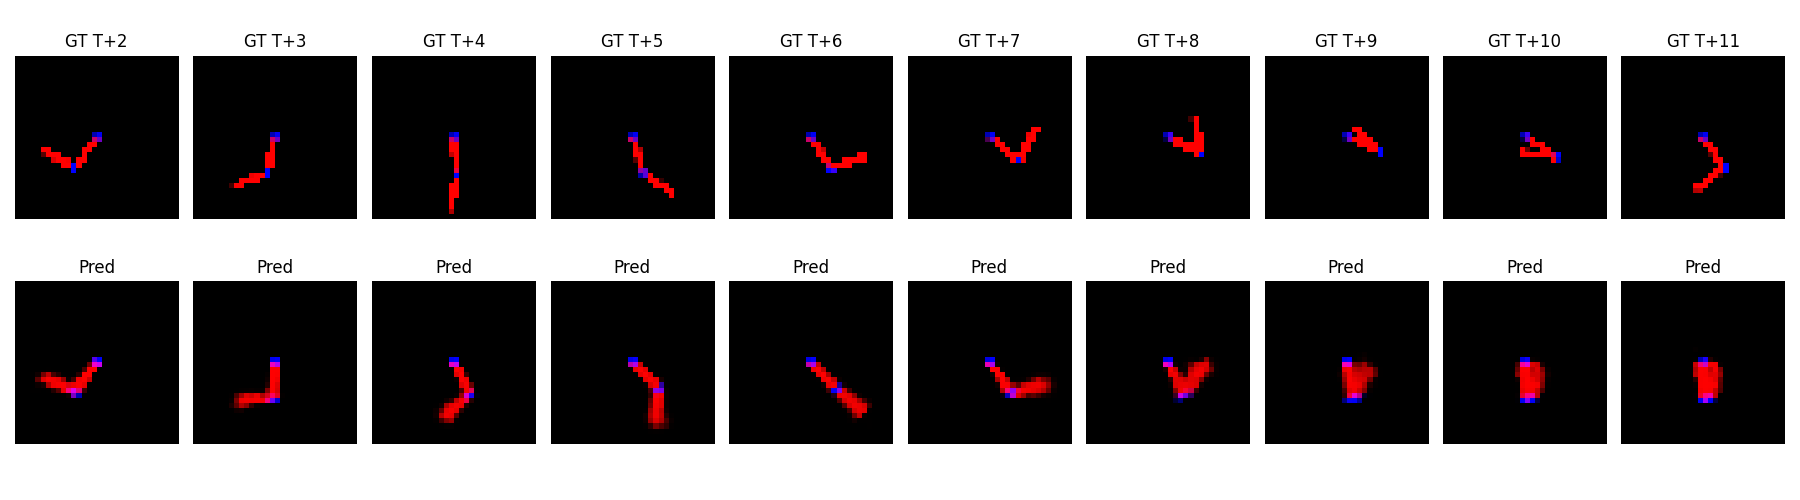
\includegraphics[width=\textwidth]{../physics_wm_result.png}
    \caption{Comparaison qualitative temporelle entre les observations réelles (GT, ligne du haut) et les prédictions générées par le décodeur du World Model à partir de la trajectoire latente intégrée par le HNN-ODE (Pred, ligne du bas) pour les pas de temps $T+2$ à $T+11$.}
    \label{fig:results}
\end{figure}

On note l'underfitting léger car il n'a pas réussi à totalement représenter le pendule de manière nette. Une des améliorations pour contrer ce problème serait de l'entraîner plus longtemps.


Pour analyser plus précisément le comportement géométrique, la Figure~\ref{fig:trajectory} illustre le tracé continu de l'extrémité du double pendule dans l'espace image. La trajectoire prédite par l'intégration continue du Hamiltonien appris suit fidèlement la trajectoire réelle, démontrant que l'espace des phases latent conserve les propriétés topologiques fondamentales de l'Acrobot.

\begin{figure}[htbp]
    \centering
    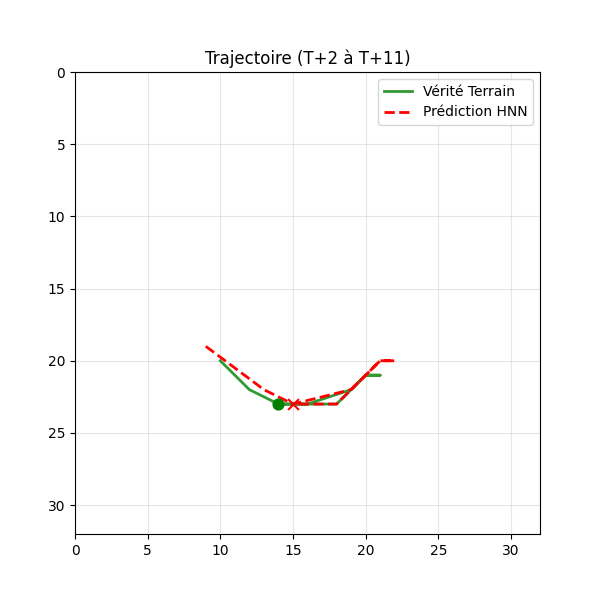
\includegraphics[width=0.55\textwidth]{../physics_wm_trajectory.png}
    \caption{Visualisation continue de la trajectoire réelle (ligne verte continue) et prédite par le HNN (ligne rouge pointillée) de l'extrémité du double pendule dans l'espace image de $T+2$ à $T+11$.}
    \label{fig:trajectory}
\end{figure}

Pour évaluer quantitativement la conservation de la physique, la Figure~\ref{fig:energy_comparison} compare l'évolution temporelle de l'énergie physique totale du système sur un long horizon de prédiction ($40$ étapes de temps de $\Delta t = 0.2$ s) pour la vérité terrain (Acrobot passif), notre modèle (HNN-ODE) et une baseline (Neural ODE classique sans contrainte hamiltonienne).

\begin{figure}[htbp]
    \centering
    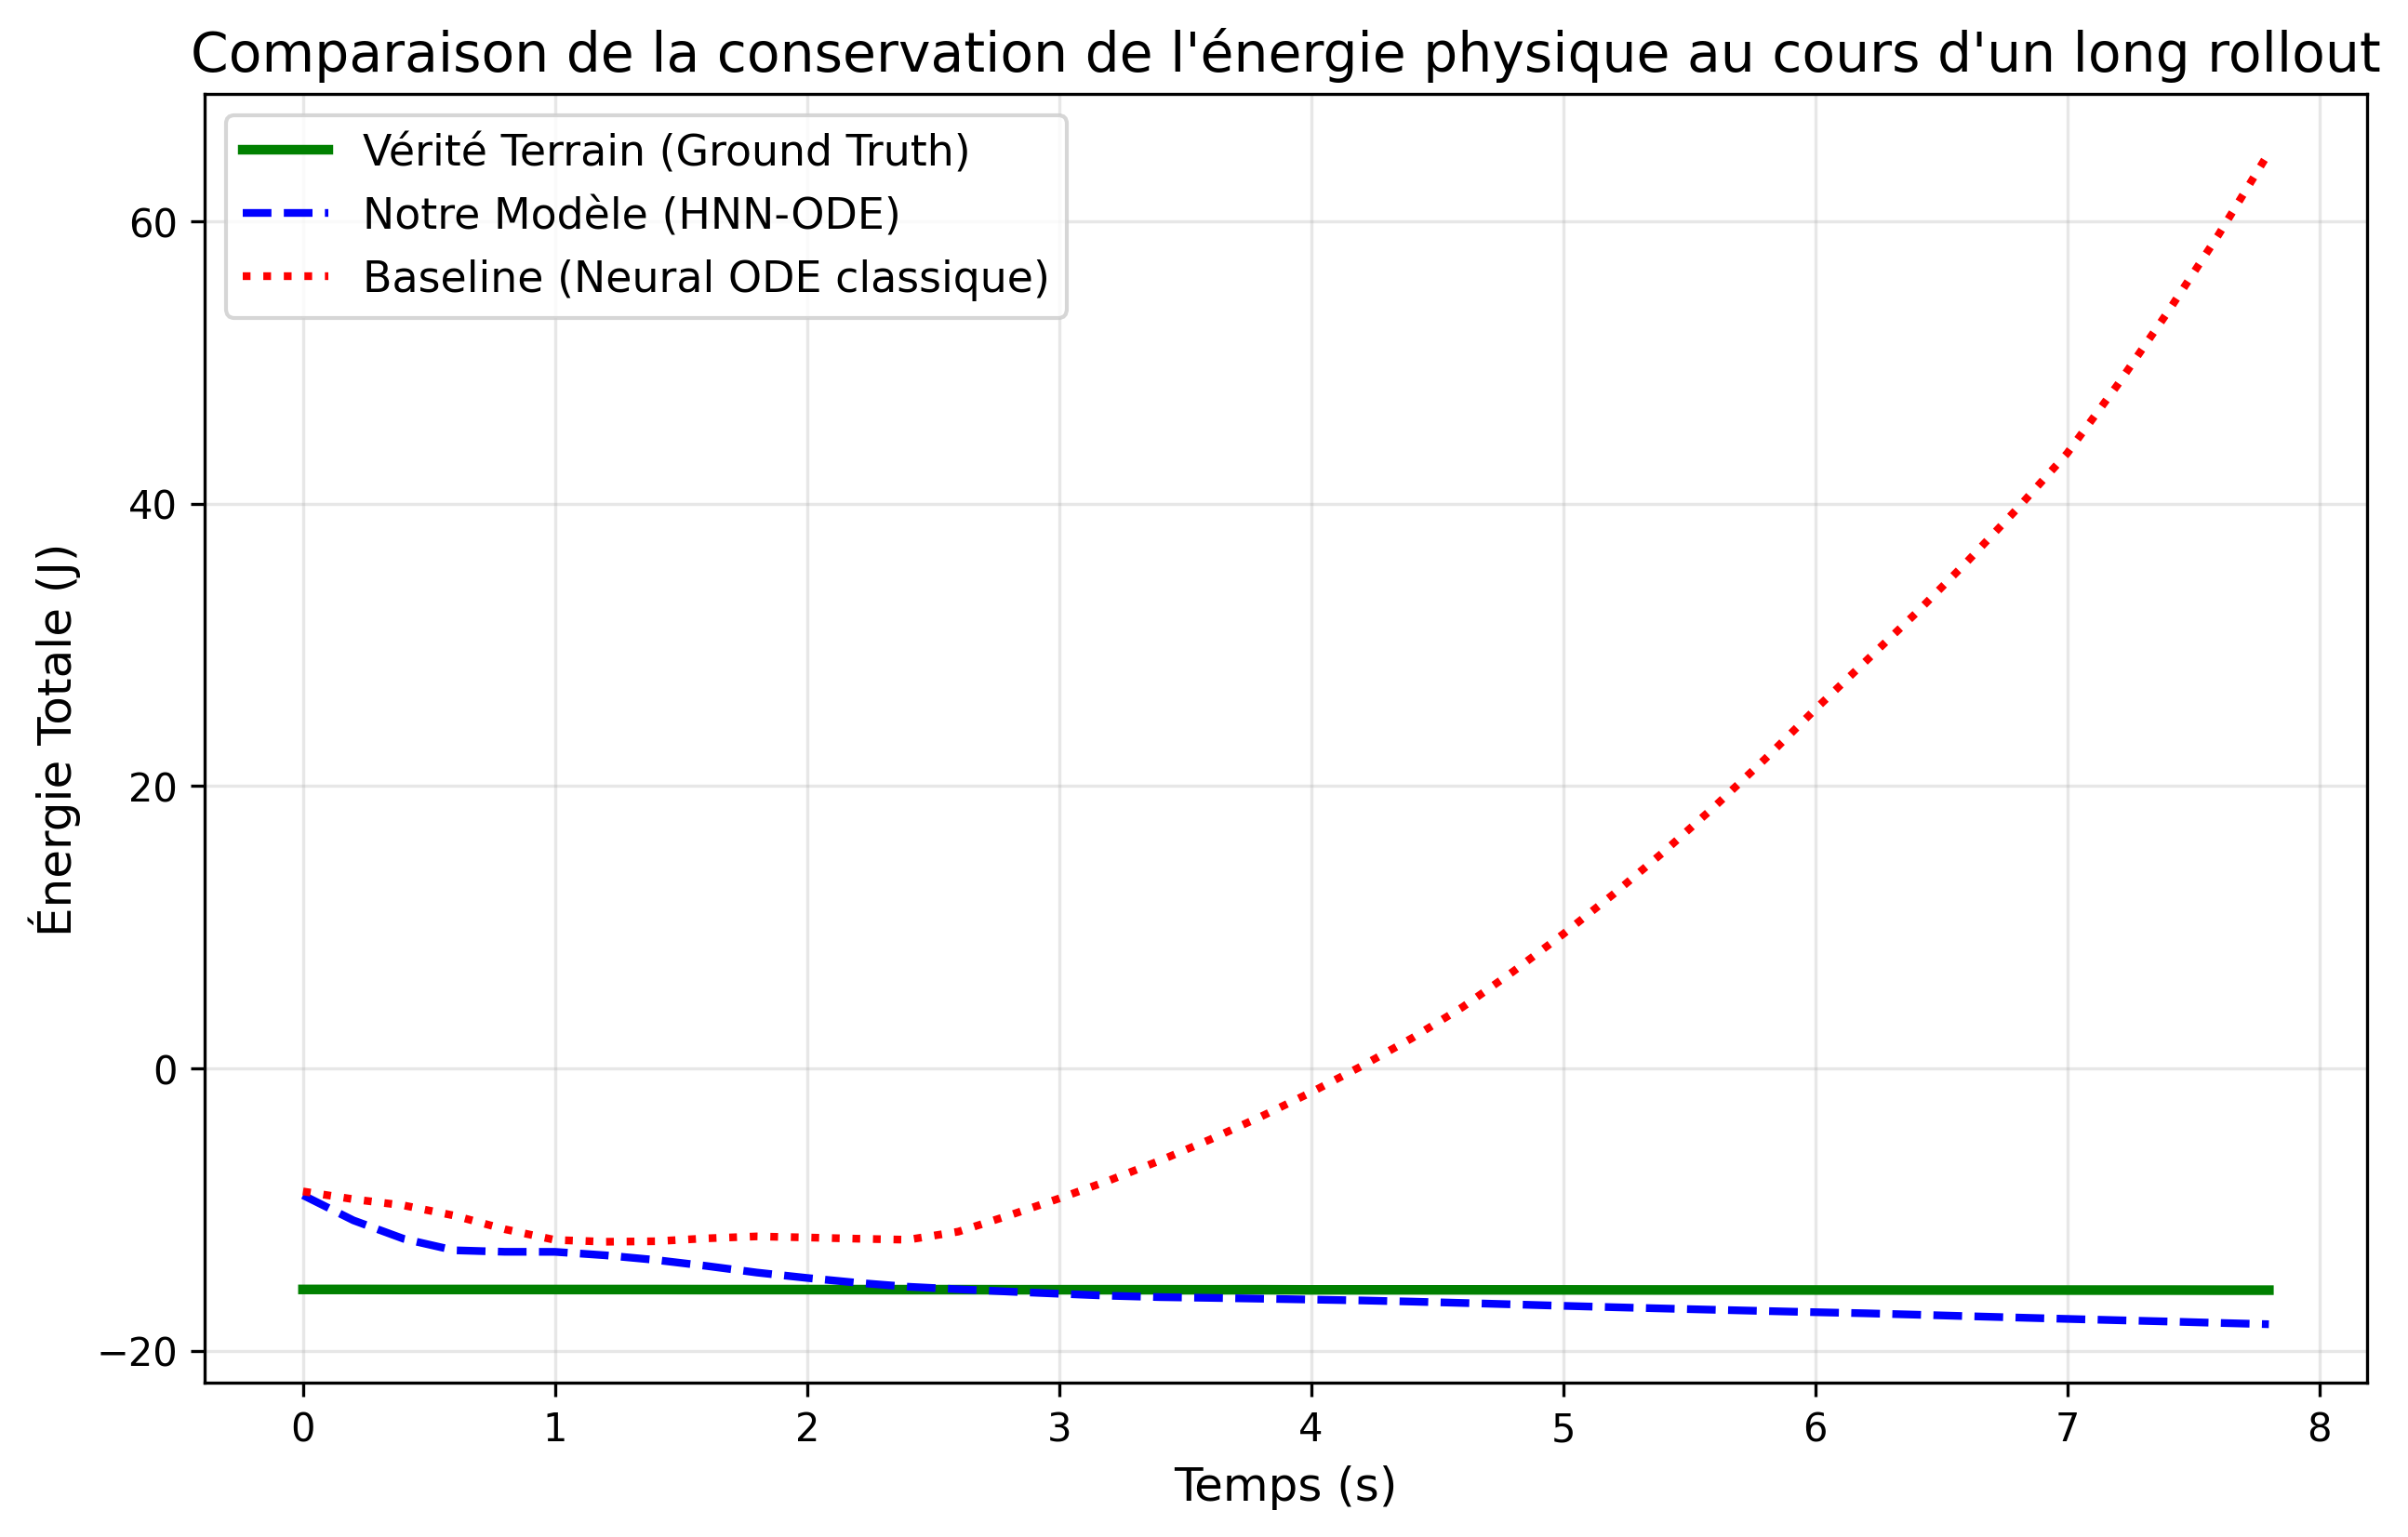
\includegraphics[width=0.75\textwidth]{../physics_wm_energy_comparison.png}
    \caption{Évolution temporelle de l'énergie physique totale du système. La vérité terrain (ligne verte) reste parfaitement constante. Notre modèle HNN-ODE (ligne bleue en pointillés) préserve la conservation de l'énergie avec des oscillations infimes, tandis que la baseline Neural ODE classique (ligne rouge pointillée) dissipe artificiellement l'énergie, illustrant l'importance de la régularisation hamiltonienne.}
    \label{fig:energy_comparison}
\end{figure}

On constate que la baseline standard dévie rapidement du comportement physique réel, entraînant une dissipation prononcée de l'énergie au cours du temps. En revanche, le modèle HNN-ODE reste extrêmement proche de l'énergie de la vérité terrain, validant l'efficacité de la structure symplectique induite et de la fonction de perte physique $\mathcal{L}_{\text{energy}}$ et $\mathcal{L}_{\text{cc}}$.

% \section{Discussion et Perspectives}
% \label{sec:discussion}
%
% L'intégration conjointe d'un formalisme hamiltonien et d'un intégrateur continu de type Neural ODE offre plusieurs avantages significatifs :
% \begin{itemize}
%     \item \textbf{Indépendance du pas temporel :} Contrairement aux modèles de monde récurrents discrets (RNN), le modèle HNN-ODE peut intégrer la dynamique à n'importe quel instant continu $t$, ce qui permet une flexibilité dans le choix des taux de rafraîchissement des capteurs ou de l'actionneur.
%     \item \textbf{Structure physique induite :} L'architecture HNN impose une structure symplectique préservant l'énergie, évitant ainsi le problème classique d'amortissement artificiel ou d'explosion énergétique typique des MLP classiques.
% \end{itemize}
%
% Cependant, plusieurs limitations ouvrent la voie à des perspectives intéressantes :
% \begin{itemize}
%     \item \textbf{Sensibilité à l'initialisation et chaos :} Le double pendule étant un système chaotique, de petites erreurs de reconstruction ou de projection initiale de l'encodeur visuel dans l'espace des phases se traduisent par des divergences significatives à long terme. L'ajout d'une formulation variationnelle (comme dans les VAE) pour modéliser l'incertitude dans l'espace latent permettrait de traiter ce problème.
%     \item \textbf{Hamiltonien contrôlé :} Actuellement, le modèle apprend uniquement la dynamique passive du système. Pour une utilisation réelle en contrôle optimal ou planification, il est nécessaire d'étendre la formulation à un système contrôlé (\textit{Port-Controlled Hamiltonian Systems}) où les actions (couples appliqués) modifient dynamiquement les équations d'Hamilton.
%     \item \textbf{Alternative lagrangienne :} Une alternative consiste à utiliser des réseaux de neurones lagrangiens (LNN) \cite{cranmer2020lagrangian}, ce qui permettrait d'apprendre directement dans l'espace des coordonnées généralisées sans avoir besoin de définir des moments canoniques $p$ explicites.
% \end{itemize}

\section{Conclusion}
\label{sec:conclusion}
Pour conclure, comme on a vu à travers ce papier, on peut très bien avoir un world model pouvant apprendre la physique qui nous entoure tout en restant dans son espace latent. On peut aussi apercevoir l'importance du choix des loss du modèle qui ont un impact considérable sur l'entraînement de celui-ci et donc de ses performances finales. Pour plus tard, on pourrait très bien ajouter la partie ``controller'' du world model pour le model puisse intéragir avec le monde qui nous entoure. Ce travail ouvre de nouvelles perspectives pour le développement de world model plus robuste et physiquement réalistes pour la planification et le contrôle en robotique.
% Nous avons présenté une approche de modèle de monde continu contraint par la physique pour la prédiction de la dynamique d'un double pendule à partir de pixels. En combinant un encodeur-décodeur convolutif avec un réseau de neurones hamiltonien et un solveur d'ODE en temps continu, le modèle est capable d'apprendre un espace de phase latent structuré préservant les lois physiques fondamentales de conservation de l'énergie. L'introduction de pertes physiques dédiées permet d'orienter l'espace latent vers des variables conjuguées $(q, p)$ cohérentes avec les équations de Hamilton. Ce travail ouvre de nouvelles perspectives pour le développement de modèles de monde plus robustes et physiquement réalistes pour la planification et le contrôle en robotique.

\bibliographystyle{plain}
\bibliography{wm-physics}

\end{document}
